\documentclass[aspectratio=1610]{beamer}
\usetheme{boxes}
\usecolortheme{crane}
\usepackage{amsmath,amsfonts}
\usepackage{algpseudocode}
\usepackage{multicol}
\usepackage{pgfplots}
\pgfplotsset{compat=1.15}
\usepackage{mathrsfs}
\usetikzlibrary{arrows}


%-------------------------------------------------------------------
%	 TITLE SLIDE
%-------------------------------------------------------------------


\begin{document}

% -------------------------------------------------------------------
% Lesson 3
% -------------------------------------------------------------------
\section{Data Structures and Algorithms}

\begin{frame}
\begin{center}
\Huge Lesson 3\\~\\
\textbf{Data Structures and Algorithms DSA}
\end{center}
\end{frame}



\begin{frame}
\frametitle{Lesson 3}

\Huge In this lesson we will talk about:
 \alert{data structures, sorting, searching, string matching algorithms}
\end{frame}



\begin{frame}{Lesson 3}{}
\begin{center}
\Huge \textbf{Data Structures}
\end{center}
\end{frame}


\begin{frame}{Lesson 3}{}
\Huge{What is a data structure?}\\~\\
\includegraphics[scale=0.80]{Images/ds}
\end{frame}



\begin{frame}{Lesson 3}{}
\LARGE
\textbf{Data Structures}\\~\\
\begin{itemize}
    \item How to \textbf{organize} data
    \item For \textbf{efficient} access
\end{itemize}

Its a collection of data values, and the relationships among these values
\end{frame}


\begin{frame}{Lesson 3}{}
\LARGE
\textbf{Sets}\\~\\
The basic, fundamental data structure: \{1,2,4,51,9\}
\begin{itemize}
    \item mathematical set
    \item unchanging
    \item contains a fixed number of elements
\end{itemize}

\end{frame}



\begin{frame}{Lesson 3}{}
\LARGE
\textbf{Sets}\\~\\
As mathematical sets are unchanging, sets which are manipulated by algorithms are dynamic. Can change in size, grow or shrink basically change over the time. 

\begin{itemize}
    \item static, 5 elements \{1,2,4,51,9\}
    \item dynamic, can add or remove more elements
\end{itemize}

\end{frame}



\begin{frame}{Lesson 3}{}
\Huge{What is a set?}\\~\\
\end{frame}


\begin{frame}{Lesson 3}{}
\LARGE
\textbf{Sets}\\~\\
\begin{itemize}
    \item The empty set \{\}
    \item Natural numbers: $\mathbb{N} = \{0, 1, 2, 3, \ldots\}$
    \item Natural numbers except 0: $\mathbb{N^*} = \{1, 2, 3, \ldots\}$
    \item Integers: $\mathbb{Z} = \{\ldots, -3, -2-, -1, 0, 1, 2, 3, \ldots\}$
    \item Positive integers: $\mathbb{Z_+} = \{0, 1, 2, 3, \ldots\}$
\end{itemize}
\end{frame}


\begin{frame}{Lesson 3}{}
\LARGE
\textbf{Basic Operations on Sets}\\~\\
\begin{itemize}
    \item insert
    \item delete
    \item test if the element belongs to a set or not 
\end{itemize}

A dynamic set which supports all these basic operations is a dictionary
\end{frame}




\begin{frame}
\begin{center}
\Huge
\begin{quote}
\textbf{"Todays software has grown by evolution, not by intelligent design"}
\begin{flushright}
{--- Leslie Lamport}	
\end{flushright}
\end{quote}
\end{center}
\end{frame}



\begin{frame}{Lesson 3}{}
\LARGE
\begin{center}
   Start with a \textbf{smart design}, at the specification level, by selecting the \textbf{right data structures} to organize and access \textbf{efficiently} your data.
\end{center}
\end{frame}



\begin{frame}{Lesson 1}{}
\begin{center}
\Huge \textbf{Data Structures}
\end{center}
\end{frame}

\begin{frame}{Lesson 2}{}
\Huge
 An algorithm is \textbf{NOT} a computer program. It is an abstraction
 \end{frame}



\begin{frame}{Lesson 1}{}
\LARGE
\textbf{What is an algorithm?}\\~\\

\begin{center}

\tikzset{every picture/.style={line width=0.75pt}} %set default line width to 0.75pt        

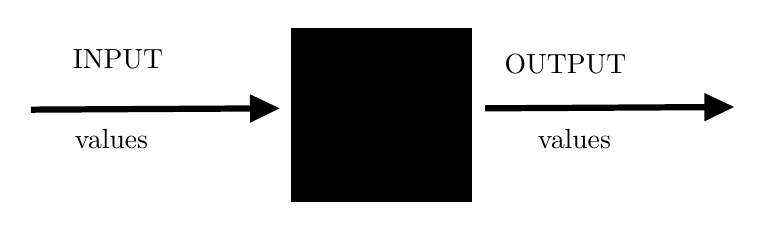
\begin{tikzpicture}[x=0.75pt,y=0.75pt,yscale=-1,xscale=1]
%uncomment if require: \path (0,171); %set diagram left start at 0, and has height of 171

%Shape: Rectangle [id:dp3842912892539916] 
\draw  [fill={rgb, 255:red, 0; green, 0; blue, 0 }  ,fill opacity=1 ][line width=2.25]  (349,57) -- (433,57) -- (433,138) -- (349,138) -- cycle ;
%Straight Lines [id:da6734653265949071] 
\draw [line width=2.25]    (440.9,94.36) -- (555.8,93.74) ;
\draw [shift={(560.8,93.71)}, rotate = 179.69] [fill={rgb, 255:red, 0; green, 0; blue, 0 }  ][line width=0.08]  [draw opacity=0] (14.29,-6.86) -- (0,0) -- (14.29,6.86) -- cycle    ;
%Straight Lines [id:da6306489033059055] 
\draw [line width=2.25]    (222,95) -- (336.9,94.38) ;
\draw [shift={(341.9,94.36)}, rotate = 179.69] [fill={rgb, 255:red, 0; green, 0; blue, 0 }  ][line width=0.08]  [draw opacity=0] (14.29,-6.86) -- (0,0) -- (14.29,6.86) -- cycle    ;


% Text Node
\draw (241,65) node [anchor=north west][inner sep=0.75pt]   [align=left] {INPUT};
% Text Node
\draw (242,103) node [anchor=north west][inner sep=0.75pt]   [align=left] {values};
% Text Node
\draw (449,67) node [anchor=north west][inner sep=0.75pt]   [align=left] {OUTPUT};
% Text Node
\draw (465,103) node [anchor=north west][inner sep=0.75pt]   [align=left] {values};

\end{tikzpicture}

$\overbrace{\hbox{Executes in a finite time}}^{\hbox{}}$

\end{center}

Sequence of computational steps that transform the input into the output

\end{frame}








\begin{frame}
\begin{center}
\Huge
\begin{quote}
\textbf{"If our software is buggy, what does
that say about its security?"}
\begin{flushright}
{--- Prof. Robert H. Morris}
\end{flushright}
\end{quote}
\end{center}
\end{frame}


\begin{frame}[plain,noframenumbering]
\makebox[\linewidth]{\includegraphics[width=\paperwidth]{Images/outage1}}
\end{frame}

\begin{frame}[plain,noframenumbering]
\makebox[\linewidth]{\includegraphics[width=\paperwidth]{Images/outage2}}
\end{frame}

\begin{frame}[plain,noframenumbering]
\makebox[\linewidth]{\includegraphics[width=\paperwidth]{Images/outage3}}
\end{frame}

\begin{frame}{Lesson 2}{}
\Huge
\center
    \textbf{What can we do about it?} 
\end{frame}



\begin{frame}{Lesson 2}{}
\Huge
\begin{center}
   Start with a \textbf{smart design} at the specification level
\end{center}
\end{frame}


\begin{frame}{Lesson 2}{}
\begin{center}
\Huge\textbf{Software Specifications}
\end{center}
\end{frame}


\begin{frame}{Lesson 2}{}
\Huge{What is a specification?}
\includegraphics[scale=0.52]{Images/specs}
\end{frame}


\begin{frame}{Lesson 2}{}
\Huge{What is a functional specification?}
\includegraphics[scale=0.46]{Images/funcspecs0}
\end{frame}


\begin{frame}{Lesson 2}{}
\huge
    A \textbf{functional software specification} is a
    \alert{written} description of what our program is supposed to do.
\end{frame}


\begin{frame}{Lesson 2}{}
\includegraphics[scale=0.41]{Images/funcspecs}
\end{frame}



\begin{frame}{Lesson 2}{}
\LARGE
\textbf{How can we write the specification?}\\~\\
\begin{itemize}
    \item English. Finnish. Chinese
    \item Graphical diagrams. Drawing
    \item Technical sketches. Mockups
\end{itemize}
\end{frame}


\begin{frame}{Lesson 2}{}
\LARGE
\textbf{Functional specification}\\~\\
Helps us to understand what our program will do. It’s highly important to write first a specification of our program \alert{before}  implementing and developing anything.
\end{frame}




\begin{frame}{Lesson 2}{}
\LARGE
    \textbf{The specification -- what our program does.}\\~\\
  
\textbf{But how should we describe this specification? How can we be precise? What does it mean to be precise?}
\end{frame}



\begin{frame}{Lesson 2}{}
\begin{center}
\Huge
	Imprecision can lead to \alert{\textbf{ERRORS!}}
\end{center}
\end{frame}


\begin{frame}{Lesson 2}{}
\LARGE
\textbf{Precise specifications}\\~\\
Its difficult to be precise using English or Chinese. Thats why in science and engineering precise specifications have adopted basic maths to describe the specifications.
\end{frame}


\begin{frame}{Lesson 2}{}
\LARGE
\textbf{Basic math}\\~\\
Elementary mathematics. Propositional logic.
\end{frame}


\begin{frame}{Lesson 2}{}
\LARGE
\textbf{Propositional Logic}\\~\\
\includegraphics[scale=0.54]{Images/basiclogic}
\end{frame}


\begin{frame}{Lesson 2}{}
\LARGE
\textbf{Propositional Logic, cont.}
\includegraphics[scale=0.55]{Images/basiclogic2}
\end{frame}



\begin{frame}{Lesson 2}{}
\LARGE
\textbf{Formal methods}\\~\\
\includegraphics[scale=0.53]{Images/fm}
\end{frame}


\begin{frame}{Lesson 2}{}
\LARGE
\textbf{Specifications using formal methods}\\~\\
\includegraphics[scale=0.53]{Images/fms}
\end{frame}


\begin{frame}{Lesson 2}{}
\LARGE
    Formal verification is the use of software tools to prove properties of a formal specification, or to prove that a formal model of a system implementation satisfies its specification.\\~\\
\textbf{Once a formal specification has been developed, the specification may be used as the basis for proving properties of the specification.}
\end{frame}

\begin{frame}{Lesson 2}{}
\LARGE
\textbf{Why maths?}\\~\\
\begin{itemize}
    \item Quantify output behavior
    \item Predict behavior of systems as design time
    \item Understand safety margins
    \item Understand system interactions
\end{itemize}
\end{frame}


\begin{frame}{Lesson 2}{}
\LARGE
    \textbf{Verification: Are we building the product right?}

\end{frame}

\begin{frame}{Lesson 2}{}
\LARGE
    \textbf{Validation: Are we building the right product?}
\end{frame}

\begin{frame}{Lesson 2}{}
\LARGE
"Building the product right" checks that the specifications are correctly implemented by the system while "building the right product" refers back to the user's needs. Ideally, formal methods provide a mathematical guarantee that software meets its specifications.
\end{frame}


\begin{frame}{Lesson 2}{}
	\Huge Industry
\end{frame}


\begin{frame}[plain,noframenumbering]
\makebox[\linewidth]{\includegraphics[width=\paperwidth]{Images/fmaws2}}
\end{frame}

\begin{frame}{Lesson 2}{}
\LARGE
\textbf{Industry: Amazon, Microsoft, NASA, ESA, Intel}\\~\\
\includegraphics[scale=0.18]{Images/fmaws}
\includegraphics[scale=0.25]{Images/fmms}
\end{frame}





%\begin{frame}{Lesson 2}{}
%\LARGE
%\textbf{}\\~\\
%A computer system differs from the systems traditionally studied by 
% scientists because we can
%pretend that its state changes in discrete steps. So, we represent the 
%execution
%of a system as a sequence of states. Formally, we define a behavior to be 
%a
%sequence of states, where a state is an assignment of values to 
%variables. We
%specify a system by specifying a set of possible behaviors—the ones 
%representing
%a correct execution of the system

\end{document}

